\begin{DensePanel}{228mm}{4}{SAFE ALONE CAN FAIL TOGETHER}
  {\DenseBody Two retuned sites close a loop through the grid, $P=K_{ij}K_{ji}$ with $K_{ij}=(I+H_{ii})^{-1}H_{ij}$:\par}
  {\DenseEq\color{IASBlue}\[
    \frac{\det F\,\det F_0}{\det F_i\,\det F_j}=\det(I-P)
  \]}
  \vspace{-2mm}
  \begin{center}
    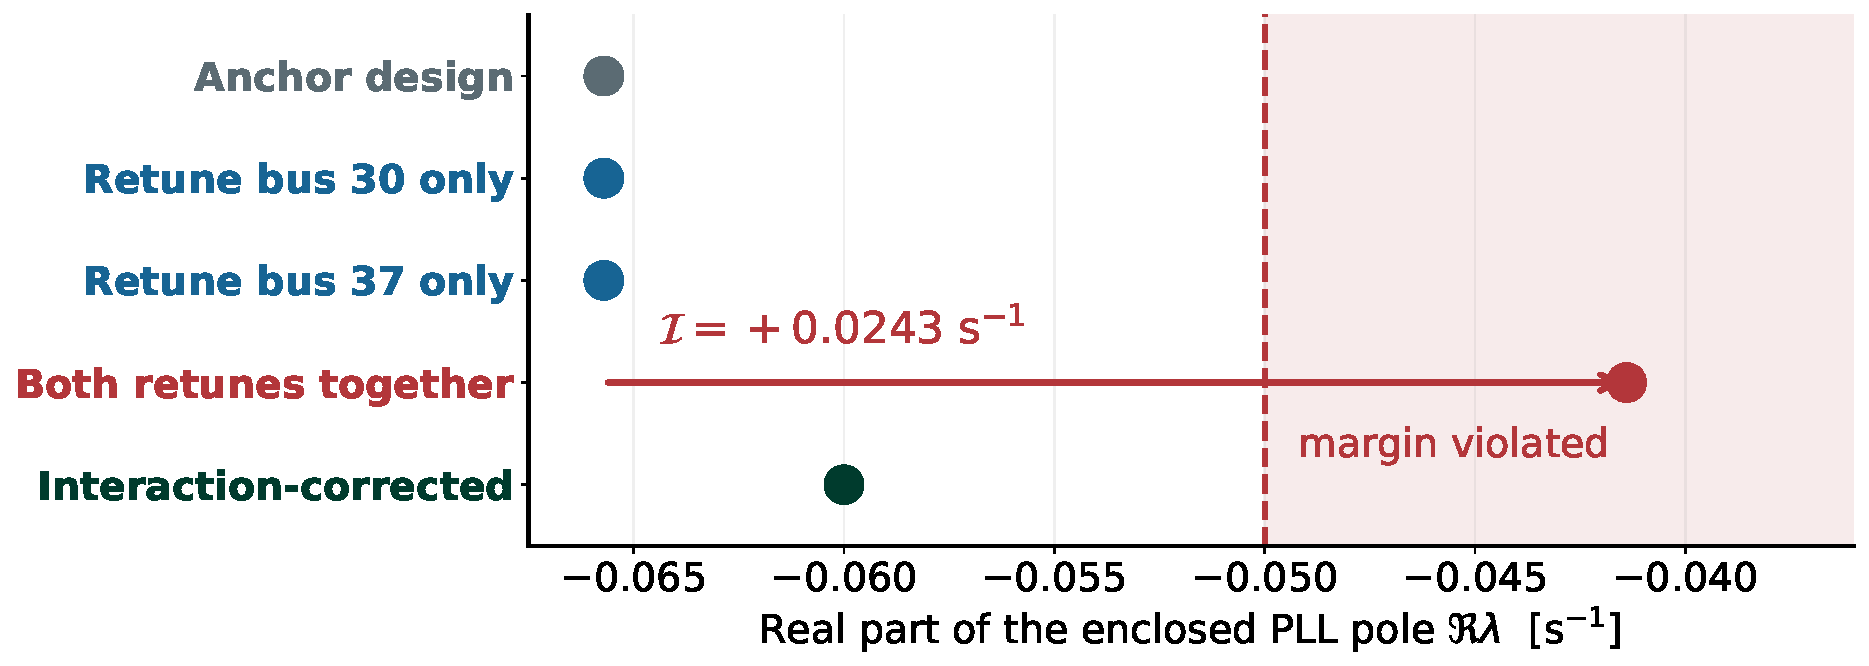
\includegraphics[width=262mm,height=86mm,keepaspectratio]{generated/figures/decision.pdf}
  \end{center}
  \vspace{-1mm}
  {\DenseSmall Buses 30 and 37 each hold the decay at $-0.0657\ \mathrm{s^{-1}}$; together $-0.0414$, past the $-0.05$ margin. Interaction $+0.0243\pm4\times10^{-7}$, interval-certified. A fixed-point budget restores $-0.060$ in 11 updates; 5 of 5 events.\par}
  \vspace{1mm}
  {\DenseSmall\color{IASGray} Matching the full complex pole instead composes (0 of 230 failures).\par}
\end{DensePanel}
